\documentclass[10pt,a4paper]{report}

% Diff�rentes options pour la classe :
% - taille de la fonte    : 10pt, 11pt, 12pt
% - recto ou recto-verso    : oneside, twoside
% - stade de d�veloppement    : draft, final

% Chargement d'extensions
%\usepackage[latin1]{inputenc}    % Pour utiliser les lettres accentu�es
\usepackage[francais]{babel}    % Pour la langue fran�aise

%\usepackage[english,francais]{babel}
\usepackage[latin1]{inputenc}    % Pour utiliser les lettres accentu�es

%\usepackage[utf8]{inputenc}
\usepackage[T1]{fontenc}
\usepackage[pdftex]{graphicx}
\usepackage{setspace}
%\usepackage{hyperref}
\usepackage[french]{varioref}
\usepackage{fancyhdr}
\usepackage{color}
\usepackage{colortbl}
\usepackage{amsmath}


\pagestyle{fancy}
\fancyhead[L]{ISTIC}
\fancyhead[C]{}
\fancyhead[R]{\rightmark}


\fancyfoot[L]{intitul� du stage}
\fancyfoot[C]{}
\fancyfoot[R]{\textbf{page \thepage}}


% D�but du document
\begin{document}


\begin{titlepage}
%\maketitle



\begin{center}
Tunisian republic
Ministry of Higher Education and Scientific Research

\begin{figure}[!ht]
\centering

\includegraphics [width =3cm]{ucar.png}
\end{figure}

Carthage University

\vspace{1cm}
\begin{figure}[!ht]
\centering

\includegraphics[width =3cm]{ISTIC.png}
\end{figure}
Higher Institute of Information and Communication Technologies

\vspace*{1cm}


\textcolor{blue}{\textbf{\Large{End Of Studies Report}}}

\vspace*{0.5cm}
\textcolor{black}{\textbf{\Huge{Project Name}}}

\vspace*{0.5cm}
\begin{figure}[!ht]
\centering

\includegraphics [width =3cm]{Sopal.png}
\end{figure}
Host Organisation::EasyTeck


\vspace*{1cm}

\textbf{\large{Students : Ouni Hani And Abdelhedi Hlel}}

\footnotesize{Fundamental Bachelor in Computer Sciences}

 
\end{center}


\begin{center}  
\vspace*{1cm}  
College year 2016 - 2017
\end{center}

\end{titlepage}

\newpage
\pagenumbering{roman}
\chapter*{D�dicaces}
\addcontentsline{toc}{chapter}{D�dicaces}

\noindent A mes parents,
\\
A mes fr�res et s\oe urs,
\\
A mes amis 


\chapter*{Remerciements}
\addcontentsline{toc}{chapter}{Remerciements}

Je tiens � remercier 


\tableofcontents    % Table des mati�res
\listoffigures        % Liste des figures
\listoftables        % Liste des tableaux
\newpage
\pagenumbering{arabic}
\chapter*{Introduction G�n�rale}
\addcontentsline{toc}{chapter}{Introduction G�n�rale}

Ce document vise � aider les �tudiants � r�diger des rapports en Latex.


\chapter{Les bases}
    %\addcontentsline{toc}{chapter}{}

\section{Introduction du chapitre}


\section{�criture d'un paragraphe simple}

Les activit�s scientifiques d'un �tudiant sont de nature � t�moigner de son d�vouement � la recherche scientifique et � l'innovation. Les candidats porteurs de projet seront favoris�s par le fait qu'ils ont une activit� pr�te � la mise en \oe uvre.


\subsection{Activit�s r�alis�es }
Le projet , � travers les formations sp�cifiques, � aider les �tudiants � mettre en \oe uvre leurs projets. Les formations offertes constituent, en effet, des stages de perfectionnement pour des candidats d�ja initi�s et ayant dans leurs actifs des formations suivies et des projets r�alis�s. 

\subsection{Lettre de motivation}
La lettre de motivation doit d�gager les attentes du candidat de la formation ou des formations � suivre. La r�daction doit pr�ciser la valeur ajout�e attendue de la participation. L'�valuation de la lettre tiendra compte de la qualit� de la r�daction et la clart� des id�es du candidat.
Cinq crit�res doivent �tre v�rifi�s pour qu'une lettre de motivation soit excellente.



\section{Insertion de figure}
%\\
\begin{figure}[h!]
	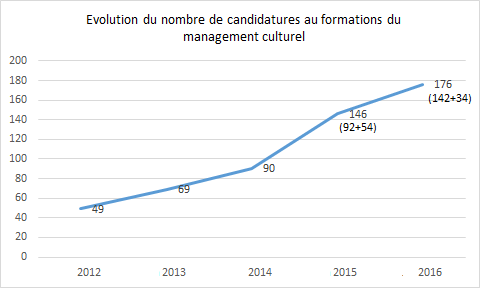
\includegraphics[width=13cm]{image3.png}
	\caption{Logo de l'entreprise SOPAL}
	\label{imag3}
\end{figure}


\section{Insertion d'un tableau}

L'attribution des points en fonction des activit�s culturelles du candidat est d�taill�e dans le tableau \ref{tab3}. 

\begin{table}
\begin{center}
\begin{tabular}{|l|l|}
\hline
\rowcolor[gray]{0.8}\bfseries Nombre de projets r�alis�s & \bfseries Points\\
\hline
>= 5 &40\\
\hline
=4 & 25\\
\hline
=3 & 15\\
\hline
=2 &10\\
\hline
=1 & 5\\
\hline
Autre & 0\\
\hline
\end{tabular}
\end{center}
\caption{Attribution des points en fonction du nombre de projets culturels r�alis�s}
\label{tab3}
\end{table}





L'attribution des points, � la lettre de motivation, en fonction du respect des crit�res sus mentionn�s est d�taill�e dans le tableau \ref{tab5}.

\begin{table}
\begin{center}
\begin{tabular}{|l|l|l|}
\hline
\rowcolor[gray]{0.8}\bfseries Respect des crit�res &\bfseries �valuation &\bfseries Points \\
\hline
C1+C2+C3+C4+C5 & Excellente &18\\
\hline
C1+C2+C3+C4 & Tr�s bien & 16\\
\hline
C1+C2+C3 & Bien & 14\\
\hline
C1+C2 & Moyen &10\\
\hline
C1 & Faible & 2\\
\hline
Autre & Insuffisant & 0\\
\hline
\end{tabular}
\end{center}
\caption{Attribution des points � la lettre de motivation en fonction du nombre de crit�res respect�s}
\label{tab5}
\end{table}



\section{Les listes}
\subsection{Les listes num�rot�es}

\begin{enumerate}

\item \textbf{C1}:La r�daction dans un langage soutenu sans erreurs d'orthographe et de grammaire,
\item \textbf{C2}:La r�daction avec des propos clairs et perspicaces,
\item \textbf{C3}:La lettre doit d�gager l'int�r�t de suivre la formation pour le candidat,
\item \textbf{C4}:Le candidat doit prouver son s�rieux et son d�sir de participer � la formation, 
\item \textbf{C5}:La Lettre doit montrer l'impact positif que pourrait avoir la formation sur la concr�tisation du projet du candidat.
\end{enumerate}

\subsection{Les listes non num�rot�es}

\begin{itemize}

\item \textbf{C1}:La r�daction dans un langage soutenu sans erreurs d'orthographe et de grammaire,
\item \textbf{C2}:La r�daction avec des propos clairs et perspicaces,
\item \textbf{C3}:La lettre doit d�gager l'int�r�t de suivre la formation pour le candidat,
\item \textbf{C4}:Le candidat doit prouver son s�rieux et son d�sir de participer � la formation, 
\item \textbf{C5}:La Lettre doit montrer l'impact positif que pourrait avoir la formation sur la concr�tisation du projet du candidat.
\end{itemize}

\section{Conclusion du chapitre}

\chapter{La bibliographie}


\section{Introduction du chapitre}


\section{Gestion les r�f�rences bibliographiques}
 
Ce document est un exemple de l'utilisation de l'environnement \texttt{thebibliography} de gestion des r�f�rences bibliographiques dans un document. trois r�f�rences sont cit�es: \textit{The \LaTeX\ Companion} 
book \cite{Johnson}, the Einstein journal paper \cite{Zoran}, et the 
Donald Knuth's website \cite{late} et \cite{texb}. 


Je cite la r�f�rence \cite{Laverdure1983}. 

Je cite la r�f�rence \cite{Agusti2003}. 

Je cite la r�f�rence \cite{Yamada2005}. 


Je cite la r�f�rence \cite{ref3}. 



\section{Conclusion du chapitre}


Je cite la r�f�rence \cite{ref4}. 



Je cite la r�f�rence \cite{WinNT}. 






\chapter{Traitement des �quations}

\section{Introduction du chapitre}


\section{Les �quations non num�rot�es}

Exemple 1

$
a = b + c
$
\vspace{1cm}

Exemple 2

$$
a = b + c
$$
\vspace{1cm}


Exemple 3

\[
a = b + c
\]


\vspace{1cm}

Exemple 4

\begin{equation*}
\centering
a = b + c
\end{equation*}




\section{Les �quations num�rot�es}

\begin{equation}
a = b + c
\end{equation}


\section{les �quations sur plusieurs lignes}

Exemple 1

\begin{multline}
a + b + c + d + e + f
+ g + h + i
= j + k + l + m + n
\end{multline}

\vspace{1cm}

Exemple 2

\begin{equation}
a = b + c + d + e + f
+ g + h + i + j
+ k + l + m + n + o + p
\label{eq:equation_too_long}
\end{equation}

\section{�quations compliqu�es}

Exemple 1

\begin{equation}
a = \sum_{k=1}^n\sum_{\ell=1}^n
\sin \bigl(2\pi \, b_k \,
c_{\ell} \, d_k \, e_{\ell} \,
f_k \, g_{\ell} \, h \bigr)
\end{equation}


\vspace{1cm}
%Exemple 2


%\begin{numcases}{}
%\dot{x} = f(x,u)

%x+\dot{x} = h(x)
%\end{numcases}

%\vspace{1cm}
%Exemple 3


%\begin{equation*}
%\int_a^b f(x) \dd x = \int_a^b
%\ln\left(\frac{x}{2}\right)
%\dd x
%\end{equation*}



\section{Conclusion du chapitre}
\chapter*{Conclusion G�n�rale et Perspectives}
\addcontentsline{toc}{chapter}{Conclusion G�n�rale et Perspectives}

Nous esp�rons que ce document vous a aid� � r�diger votre rapport convenablement.
\chapter*{Annexe 1}
\addcontentsline{toc}{chapter}{Annexe 1, Les candidats class�s par ordre alphab�tique}




\chapter*{Annexe 2}
\addcontentsline{toc}{chapter}{Annexe 2, D�tails de calcul du score}


\begin{table}
\begin{center}
\begin{tabular}{|l|l|l|l|l|l|l|}
\hline
\rowcolor[gray]{0.8}\bfseries Ordre & \bfseries Candidat& \bfseries Mathl& \bfseries Physique & \bfseries Informatique  & \bfseries Projet & \bfseries Score\\
\hline
\hline
1& & & & & & \\
\hline 
2& & & & & & \\
\hline
3& & & & & & \\
\hline
4& & & & & & \\
\hline 
5& & & & & & \\
\hline 
6& & & & & & \\
\hline 
7& & & & & & \\
\hline 
8& & & & & & \\
\hline 
9& & & & & & \\
\hline 
10& & & & & & \\
\hline 
\end{tabular}
\end{center}
\caption{D�tails de l'attribution des points}
\label{tab22}
\end{table}

\bibliographystyle{alpha}
\bibliography{Biblio}


		

    

% Fin du document
\end{document}